\section{Overview}

\begin{frame}[standout]
There are bottom-up and top-down approaches. Think: explorative anlaysis and finding patterns vs. finding something pre-defined and testing a specific hypothesis.
\end{frame}


%\begin{frame}[plain]
%\makebox[\linewidth]{
%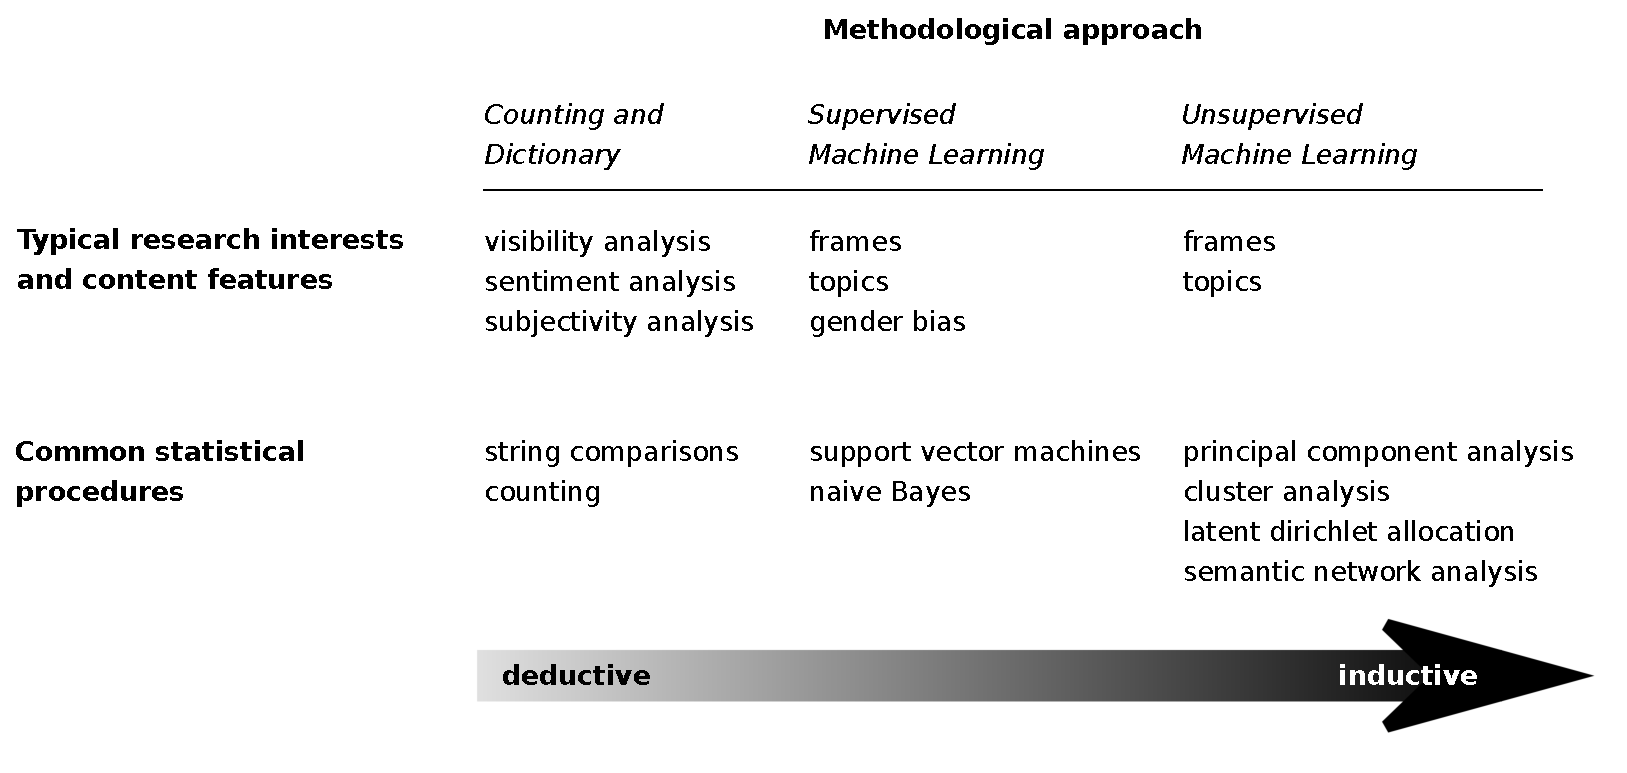
\includegraphics[width=\paperwidth,height=\paperheight,keepaspectratio]{boumanstrilling2016}}
%\cite{Boumans2016}
%
%\textbf{\textcolor{orange}{The same logic applies to non-textual data!}}
%\end{frame}









\begin{frame}{Some terminology }
\begin{columns}[t]
\column{.5\textwidth}

\begin{block}<1-4>{Supervised machine learning}
  You have a dataset with both predictor and outcome (independent and dependent variables; features and labels) --- a \emph{labeled} dataset.
  \onslide<2>{
    \footnotesize{Think of regression: You measured \texttt{x1}, \texttt{x2}, \texttt{x3} and you want to predict \texttt{y}, which you also measured}}
\end{block}

\column{.5\textwidth}

\begin{block}<3->{Unsupervised machine learning}
  You have no labels. \onslide<4>{(\footnotesize{You did not measure \texttt{y})}}\\
  \onslide<5>{\textbf{You might already know \emph{some} techniques to figure out whether \texttt{x1}, \texttt{x2},\ldots \texttt{x\_i} co-occur} \begin{itemize}
    \item Principal Component Analysis (PCA) and Singular Value Decomposition (SVD)
    \item Cluster analysis
    \item Topic modelling (Non-negative matrix factorization and Latent Dirichlet Allocation)
    \item \ldots
    \end{itemize}}
\end{block}

\end{columns}

\end{frame}


\begin{frame}{Let's distinguish four use cases\ldots}

\begin{enumerate}
\item Finding similar variables (dimensionality reduction) -- unsupervised
\item Finding similar cases (clustering) -- unsupervised
\item Predicting a continous variable (regression) -- supervised
\item Predicting group membership (classification) -- supervised
\end{enumerate}
\end{frame}


\begin{frame}[plain]
\begin{table}[]
\resizebox{\textwidth}{!}{%
\begin{tabular}{lllllll}
& x1 & x2 & x3 & x4 & x5 & y \\
case1 & \ding{110}  & \ding{110}  & \ding{110}  & \ding{110}  & \ding{110} & \ding{110} \\
case2 & \ding{110}  & \ding{110}  & \ding{110}  & \ding{110}  & \ding{110} & \ding{110}\\
case3 & \ding{110}  & \ding{110}  & \ding{110}  & \ding{110}  & \ding{110} & \ding{110}\\
case4 & \ding{110}  & \ding{110}  & \ding{110}  & \ding{110}  & \ding{110} & \ding{110}\\
\end{tabular}%
}
\end{table}
 ~ 
\end{frame}



\begin{frame}[plain]
\begin{table}[]
\resizebox{\textwidth}{!}{%
\begin{tabular}{lllllll}
& \textcolor{orange}{x1} & x2 & \textcolor{orange}{x3}& \textcolor{blue}{x4} & \textcolor{blue}{x5} & \textcolor{gray}{(y)} \\
case1 & \textcolor{orange}{\ding{110}}  & \ding{110}  & \textcolor{orange}{\ding{110}}  & \textcolor{blue}{\ding{110}} & \textcolor{blue}{\ding{110}} & \textcolor{gray}{(\ding{110})} \\
case2 & \textcolor{orange}{\ding{110}}  & \ding{110}  & \textcolor{orange}{\ding{110}}  & \textcolor{blue}{\ding{110}} & \textcolor{blue}{\ding{110}} & \textcolor{gray}{(\ding{110})} \\
case3 & \textcolor{orange}{\ding{110}}  & \ding{110}  & \textcolor{orange}{\ding{110}}  & \textcolor{blue}{\ding{110}} & \textcolor{blue}{\ding{110}} & \textcolor{gray}{(\ding{110})} \\
case4 & \textcolor{orange}{\ding{110}}  & \ding{110}  & \textcolor{orange}{\ding{110}}  & \textcolor{blue}{\ding{110}} & \textcolor{blue}{\ding{110}} & \textcolor{gray}{(\ding{110})} \\
\end{tabular}%
}
\end{table}
Dimensionality reduction: finding similar variables (features)
\end{frame}


\begin{frame}[plain]
\begin{table}[]
\resizebox{\textwidth}{!}{%
\begin{tabular}{lllllll}
& x1 & x2 & x3 & x4 & x5 & \textcolor{gray}{(y)} \\
\textcolor{orange}{case1} & \textcolor{orange}{\ding{110}}  & \textcolor{orange}{\ding{110}}  &\textcolor{orange}{\ding{110}}  &\textcolor{orange}{\ding{110}}   & \textcolor{orange}{\ding{110}} & \textcolor{gray}{(\ding{110})} \\
\textcolor{blue}{case2} & \textcolor{blue}{\ding{110}}  & \textcolor{blue}{\ding{110}}  &\textcolor{blue}{\ding{110}}  &\textcolor{blue}{\ding{110}}   & \textcolor{blue}{\ding{110}} & \textcolor{gray}{(\ding{110})} \\
\textcolor{orange}{case3} & \textcolor{orange}{\ding{110}}  & \textcolor{orange}{\ding{110}}  &\textcolor{orange}{\ding{110}}  &\textcolor{orange}{\ding{110}}   & \textcolor{orange}{\ding{110}} & \textcolor{gray}{(\ding{110})} \\
\textcolor{orange}{case4} & \textcolor{orange}{\ding{110}}  & \textcolor{orange}{\ding{110}}  &\textcolor{orange}{\ding{110}}  &\textcolor{orange}{\ding{110}}   & \textcolor{orange}{\ding{110}} & \textcolor{gray}{(\ding{110})} \\
\end{tabular}%
}
\end{table}
Clustering: finding similar cases
\end{frame}



\begin{frame}[plain]
\begin{table}[]
\resizebox{\textwidth}{!}{%
\begin{tabular}{llllllll}
& x1 & x2 & x3 & x4 & x5 & $\rightarrow$ & \textcolor{orange}{y} \\
case1 & \ding{110}  & \ding{110}  & \ding{110}  & \ding{110}  & \ding{110} & $\rightarrow$ &\textcolor{orange}{\ding{110}}  \\
case2 & \ding{110}  & \ding{110}  & \ding{110}  & \ding{110}  & \ding{110} & $\rightarrow$ &\textcolor{orange}{\ding{110}} \\
case3 & \ding{110}  & \ding{110}  & \ding{110}  & \ding{110}  & \ding{110} & $\rightarrow$ &\textcolor{orange}{\ding{110}} \\
case4 & \ding{110}  & \ding{110}  & \ding{110}  & \ding{110}  & \ding{110} & $\rightarrow$ &\textcolor{orange}{\ding{110}} \\
&&&&&&& \\
new case & \ding{110}  & \ding{110}  & \ding{110}  & \ding{110}  & \ding{110} & $\rightarrow$ &\textbf{\textcolor{orange}{?}} \\
\end{tabular}%
}
Regression and classification: learn how to predict $y$.
\end{table}
\end{frame}




\begin{frame}[plain]
\textbf{Note, again, that the \ding{110} signs can be \emph{anything}}: a person's age, the frequency of a word, the color of a pixel, a number of clicks.

\begin{table}[]
\resizebox{\textwidth}{!}{%
\begin{tabular}{lllllll}
& x1 & x2 & x3 & x4 & x5 & y \\
case1 & \ding{110}  & \ding{110}  & \ding{110}  & \ding{110}  & \ding{110} & \ding{110} \\
case2 & \ding{110}  & \ding{110}  & \ding{110}  & \ding{110}  & \ding{110} & \ding{110}\\
case3 & \ding{110}  & \ding{110}  & \ding{110}  & \ding{110}  & \ding{110} & \ding{110}\\
case4 & \ding{110}  & \ding{110}  & \ding{110}  & \ding{110}  & \ding{110} & \ding{110}\\
\end{tabular}%
}
\end{table}
\end{frame}


